\documentclass[11pt]{article}
\usepackage[margin=1in]{geometry}
\usepackage{amsfonts, amsmath, amssymb}
\usepackage[none]{hyphenat}
\usepackage{fancyhdr}
\usepackage{graphicx}
\graphicspath{ {./media/} }
\usepackage{float}
\usepackage{setspace}
\usepackage{subfig}
\usepackage[nottoc, notlot, notlof]{tocbibind}
%\usepackage{unicode-math}
\usepackage{tabularx}
\usepackage{amsmath} % for boxing equations
\usepackage[font=footnotesize]{caption}
\usepackage{listings}




\pagestyle{fancy}
\fancyhead{}
\fancyfoot{}
\fancyhead[L]{\slshape CALCULATING AREA WITH MONTE CARLO SIMULATIONS}
%\fancyhead[R]{\slshape Ben Datsko}
\fancyfoot[C]{\thepage}

\parindent 0ex
%\setlength{\parindent{4em}}
%\renewcommand{\headrulewidth}{0pt}
\renewcommand{\baselinestretch}{1.5}

\begin{document}

\begin{titlepage}
\begin{center}
\vspace*{1cm}
\Large{{IB Mathematics Analysis and Approaches HL}}\\
\Large{Internal Assessment}
\vfill
\line(1,0){400}\\[1mm]
\Large{\textbf{The Monte Carlo Method: An Unconventional Means\\of Calculating Area}}\\
%\Large{\textbf{This is a Sample Subtitle}}\\[1mm]
\line(1,0){400}\\
\vfill
\normalsize Spring 2021\\ 
\normalsize Investigation Page Count: 12\\


\end{center}
\end{titlepage}

\tableofcontents
\thispagestyle{empty}
\clearpage

\setcounter{page}{1}

\section{Introduction}
\subsection{Background}
Light is a compelling phenomenon as it is difficult to manipulate and seemingly impossible to predict. In the real world, when a light source emits a light ray that then collides with another object, the ray is scattered in infinitely many directions (Figure 1). I assumed 3D computer graphics programs like Blender, which I fiddle with regularly, approached simulating light in scenes in the same way; however, I quickly realized that would not make sense, as no computer can produce an infinite quantity of anything, including simulated light rays. Nevertheless, most 3D computer graphics programs can still produce photorealistic images, which led me to investigate how such programs calculate light. Interestingly, as opposed to performing a complex mathematical calculation for each of the one million-plus simulated light rays (which is what I hypothesized might occur), 3D graphics programs simulate a large number of randomly selected light paths and use probability to determine how a scene should be lit. In essence, areas that are hit by more of the randomly-generated light rays are brightly illuminated, whereas areas that are hit by fewer rays appear darker. Mathematicians widely regard this computational practice as the Monte Carlo method.\cite{blenderrender}\\

\begin{figure}[h]
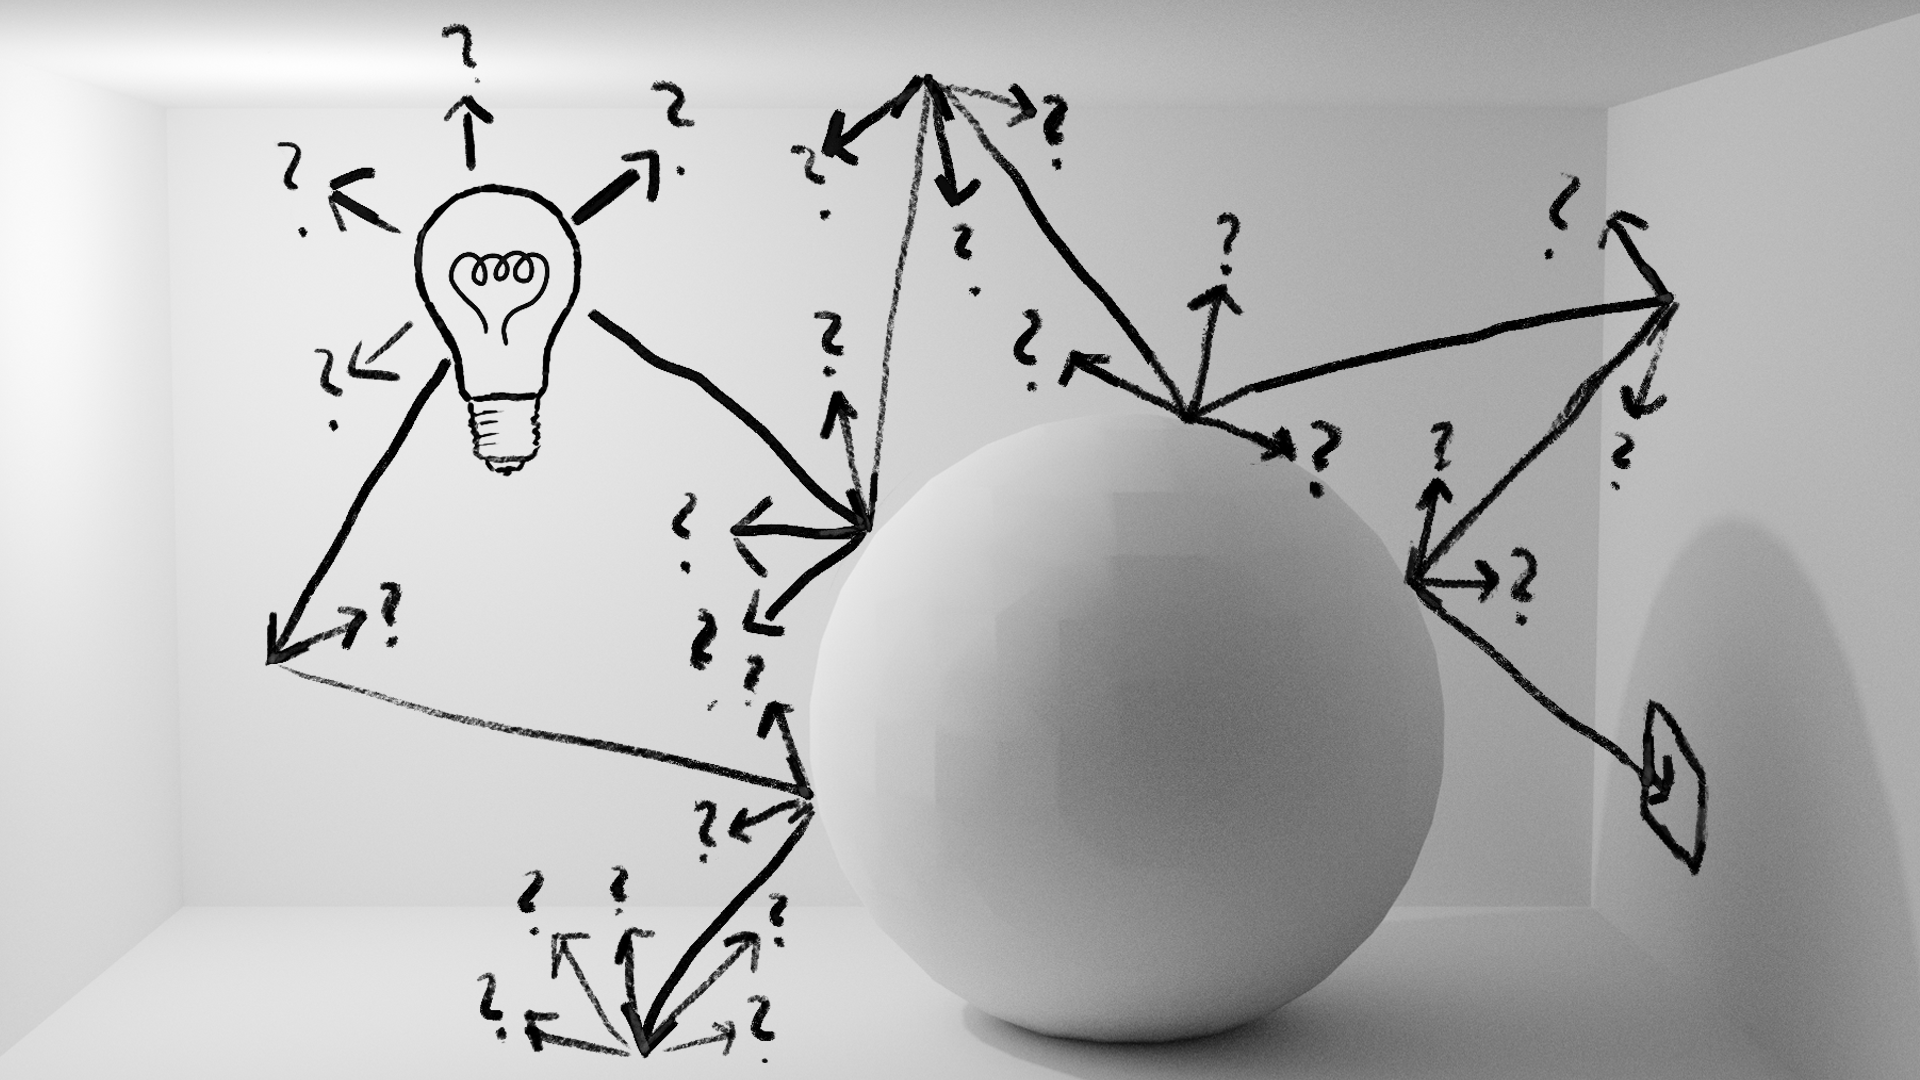
\includegraphics[scale=.15]{blackandwhite}
\centering\\
\footnotesize\centering Figure 1: An image created in Blender for the purpose of demonstrating the behavior of light paths in this investigation.
\end{figure}

\normalsize The Monte Carlo method is interesting to me as I have always solved mathematical problems with deterministic, formulaic methods, and have never thought to combine probability with numerical problems that have seemingly fixed solutions. This paper will apply the Monte Carlo method to calculating the area of shapes in Euclidean geometry. Conventional methods for solving for the area of shapes through utilizing numeric relationships and calculus are typically time-consuming and complicated, especially for irregular shapes. This investigation will evaluate whether using the Monte Carlo method to solve for the area of shapes is advantageous over conventional methods for solving.

\subsection{The Monte Carlo Method}

The Monte Carlo method, or Monte Carlo simulations, rely on repeated random sampling of a large population to obtain a representative sample of the sampled population. Reasons for how the Monte Carlo method works and why it is so effective can be provided by a real-life example of the Monte Carlo method at work in the sciences. For example, if one wanted to find the average height of all human beings, the individual would have to sample the entire human population and average all the data. However, due to the sheer size of the human population, employing this computational method would be incredibly impractical. Alternatively, a smaller sample group could be selected systematically with the Monte Carlo method to represent the entire human population. The guidelines for selecting this group are as follows:

\begin{itemize}

  \item First, samples must be selected randomly to ensure the sample group is as unbiased as possible. If the surveyor employs convenience sampling (e.g. they only survey the next 10 people they meet), the sample would still not be representative of the global population because the surveyor may happen to live in an area with especially tall or short people. Employing random sampling (randomly selecting people worldwide) to form a sample group would circumvent this issue, as well as many other issues pertaining to sample selection, which is why it is used to create unbiased samples in the Monte Carlo method.

  \item Second, the sample group must not be too small. If the heights of 5 people are measured, there is a chance that the surveyor could have coincidentally picked 5 taller or shorter people. Therefore, one can be more confident in the result of a simulation the more sample points that are gathered. In probability theory, this is referred to as the "Law of Large Numbers," and it is the primary reason why computers execute Monte Carlo simulations, as they can generate thousands of sample points in a matter of seconds.

\end{itemize}

The area of a circle and a polar rose (i.e. a rhodonea curve) will now be calculated both deterministically, as well as through the Monte Carlo method. Through comparison of the efficiency and accuracy at which the two methods calculate the area of the shapes, the mathematical and practical applications of the Monte Carlo method can be explored deeper. The area of a circle will be calculated first to demonstrate the properties of the method.

\section{The Area of a Circle}
\subsection{Deterministic Calculations}

First, a very simple deterministic calculation will be performed to solve for the area of the unit circle.
\begin{figure}[h]
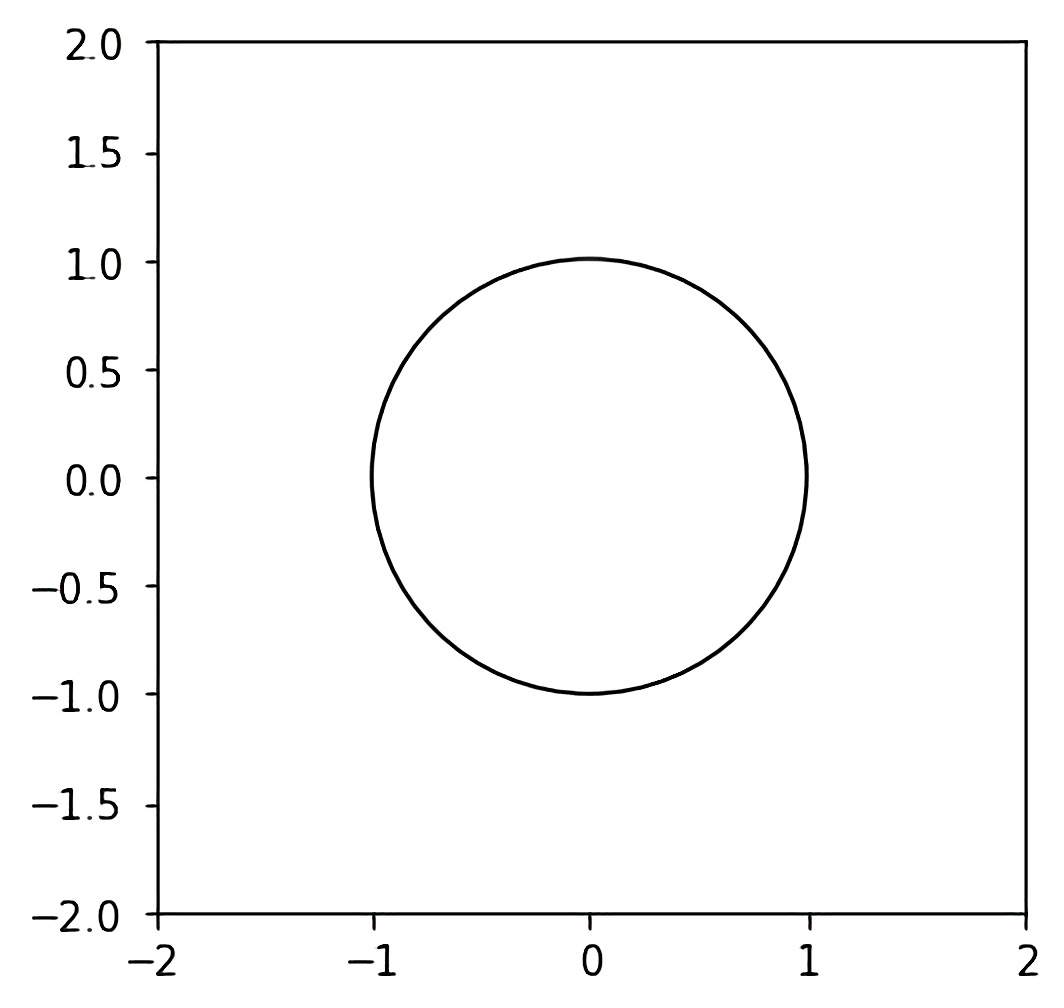
\includegraphics[scale=.2]{circle_clear}
\centering\\
\footnotesize\centering Figure 2: A circle with origin (0, 0) and radius 1. 
\end{figure}

Figure 2 provides the radius (1), origin (0, 0) of a unit circle. The equation for this circle is given by\\[-10ex]

\[(x-0)^2+(y-0)^2=1\]

The domain of possible inputs consists of the square bounded by the x and y axes, as well as the lines x=-2, x=2, y=-2, and y=2 (represented by the square outline in Figure 2). The standard area of a circle equation can now be used to solve for the exact value of the area of the unit circle:\\[-7ex]

\[A=\pi r^2=\pi 1^2 \approx \boxed{\pi \ units^2}\]
%\[ \boxed{A = 10.265} \]



\subsection{Calculating Using the Monte Carlo Method}
To calculate the area of the circle using the Monte Carlo method, I created a computer program in Python that approximates the area of a shape through performing a Monte Carlo simulation. I chose to create the program in Python because it allowed me to strengthen my programming skills (as I had never worked with Python before), and because Python can perform complex mathematical calculations far more efficiently than other popular programs used for performing Monte Carlo simulations, such as MatLab. Within my program, I included libraries such as MatPlotLib (which generates graphs) and NumPy (which implements data structures that are used to store the coordinates of shape vertices). NumPy also offers a powerful \texttt{random} library (a set of functions that generate pseudo-random numbers), as it produces values that are almost truly random. This library generates random floats uniformly in the range $[0, 1)$ using the Mersenne Twister at its core: a computational algorithm capable of generating numbers with 53 digits of precision \cite{pythongen}. However, predictability still remains in the random number generation process as a pre-programmed computer algorithm generates them to begin with. This does influence the calculations performed later in this investigation slightly, although, through following the Law of Large numbers and increasing the number of samples, this effect is mitigated to the point where it is negligible. The program itself is included under Appendix A.\\[-2ex]

The aforementioned program functions as follows: To begin, several thousand sample points, whose coordinates are randomly generated using the \texttt{random} library, are plotted across the domain. Each point's x and y coordinates are then stored in an array (i.e. a list). Then, a shape is generated in the same plane. After all sample points and the shape have been generated, the program iterates through the coordinates of every sample point in the array and tests whether it lies inside of the shape. For every point that is inside the shape, 1 is added to a counter labeled \texttt{inside\_shape}. The predicted area of the shape is then calculated by taking the percentage of all the points within the circle that lie across the domain ($ \frac{inside\_shape}{total\_sample\_points}$) and multiplying it by the area of the domain (which, in this instance, is a square with legs measuring 4 units; thus its area measures 16 units$^2$). A visual representation of the simulation is then outputted by the program (Figure 3).\\[-5ex]

%\[\frac{InsideShape}{TotalPointsAcrossDomain}*16\]


\begin{figure}[h]
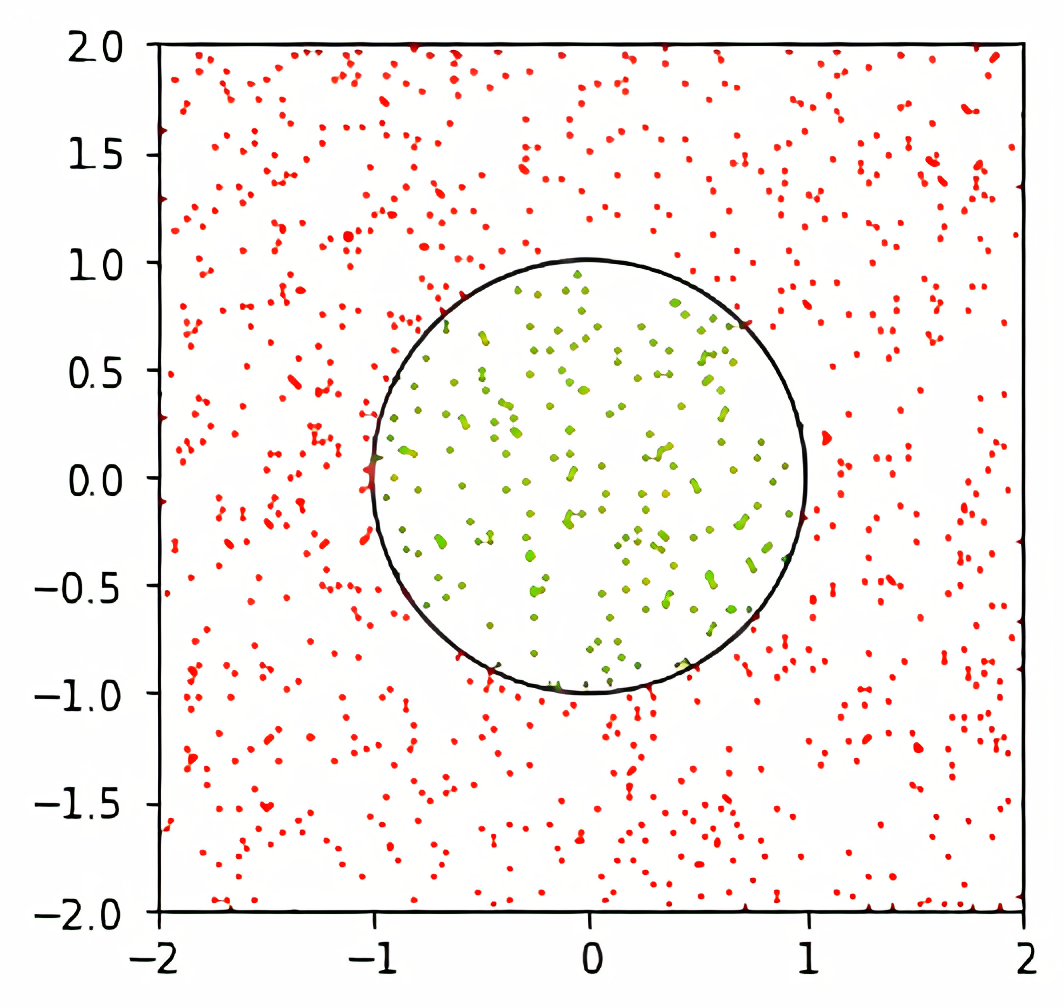
\includegraphics[scale=.19]{circle_populated}
\centering\\
\footnotesize\centering Figure 3: A Monte Carlo simulation plot with 1000 points (generated by the program).
\end{figure} 

\raggedright

\newpage
The table below lists 10 trials, each of which has a different number of generated points and predicted area for the shape. The percent error of each trial is calculated through the standard equation for percent error:\\[-3ex]

\[\frac{|Theoretical-Experimental|}{|Theoretical|}*100\]

 


\begin{table}[H]
    \centering
    \begin{tabularx}{\linewidth}{>{\centering\arraybackslash}X>{\centering\arraybackslash}X>{\centering\arraybackslash}X>{\centering\arraybackslash}X>{\centering\arraybackslash}X }
      \hline \textbf{Number of Points} & \textbf{Points in Circle} & \textbf{Percent of Domain} & \textbf{Predicted Area} & \textbf{Percent Error} \\ \hline
              5                            &	2                         & 40.0\%                      & 6.400                  & 103.72\%            \\ \hline
              10                            &	3                        & 30.0\%                      & 4.800                  & 52.789\%            \\ \hline
              20                            &	5                        & 25.0\%                      & 4.000                  & 27.324\%            \\ \hline
              50                           &	12                        & 24.0\%                      & 3.840                  & 22.231\%            \\ \hline
              100                           &	21                       & 20.9\%                      & 3.340                  & 6.3155\%            \\ \hline
              500                          &	103                       & 20.6\%                      & 3.296                  & 4.9149\%            \\ \hline
              1000                          & 201                      & 20.1\%                      & 3.216                  & 2.3684\%            \\ \hline
              10000                          & 2004                      & 20.0\%                      & 3.206                  & 2.0629\%            \\ \hline
              50000                         & 9890                      & 19.8\%                      & 3.165                  & 0.73871\%            \\ \hline
              100000                         & 19640                     & 19.6\%                      & 3.142                  & 0.02567\%            \\ \hline

    \end{tabularx}\\[2ex]
    \centering\footnotesize Table 1: Predicted area and its accuracy for a varying number of test points.
    \label{tab:data}
  \end{table}
  
It took the computer 183 seconds to generate 100,000 points. Thus, the number of sample points within each simulation is capped at 100,000 within this investigation for the sake of time, and because adding additional points would produce a negligible difference in the accuracy of the result. Additionally, the area of the unit circle is the irrational value $\pi$; therefore, attempting to attain a definite solution by proceeding further and adding additional points would be a futile effort (although it would allow one to estimate additional digits of $\pi$).\\[3ex]

Additionally, the Law of Large Numbers is supported by Table 1, as the greater the amount of points that are generated, the smaller the percent error, and thus the more accurate the prediction for area. After 100,000 points were used, the percent error became less than one third of a percent.  This clearly demonstrates that the Monte Carlo method can accurately estimate the area of shapes, although, in this instance, it did not provide a methodical advantage over the deterministic method of solving.\\


\section{The Area of a Polar Rose}
\subsection{Rationale and Background}

In the previous section, it was disadvantageous to use the Monte Carlo method to calculate the area of the circle, as it required more computing time and power than using deterministic numerical calculation. However, in the case of irregularly-shaped polygons and curved shapes, which have hundreds of degrees of freedom (dimensions), ``the curse of dimensionality dictates an exponential increase in complexity as the number of dimensions rises when using deterministic numerical integration.”\cite{dynamicprogramming} Thus, utilizing the Monte Carlo method to calculate the area of such irregular shapes could circumvent the aforementioned ``exponential increase in computational time." \\[3ex]

To demonstrate this, the area of a polar rose (Figure 4) will be calculated through both numerical integration and the Monte Carlo method. The polar rose was selected for this investigation because calculating its area is complex enough to where solving through deterministic means is burdensome, but not ridiculously complicated. 


\begin{figure}[h]%
    \centering
    \subfloat[\centering Cartesian Plane]{{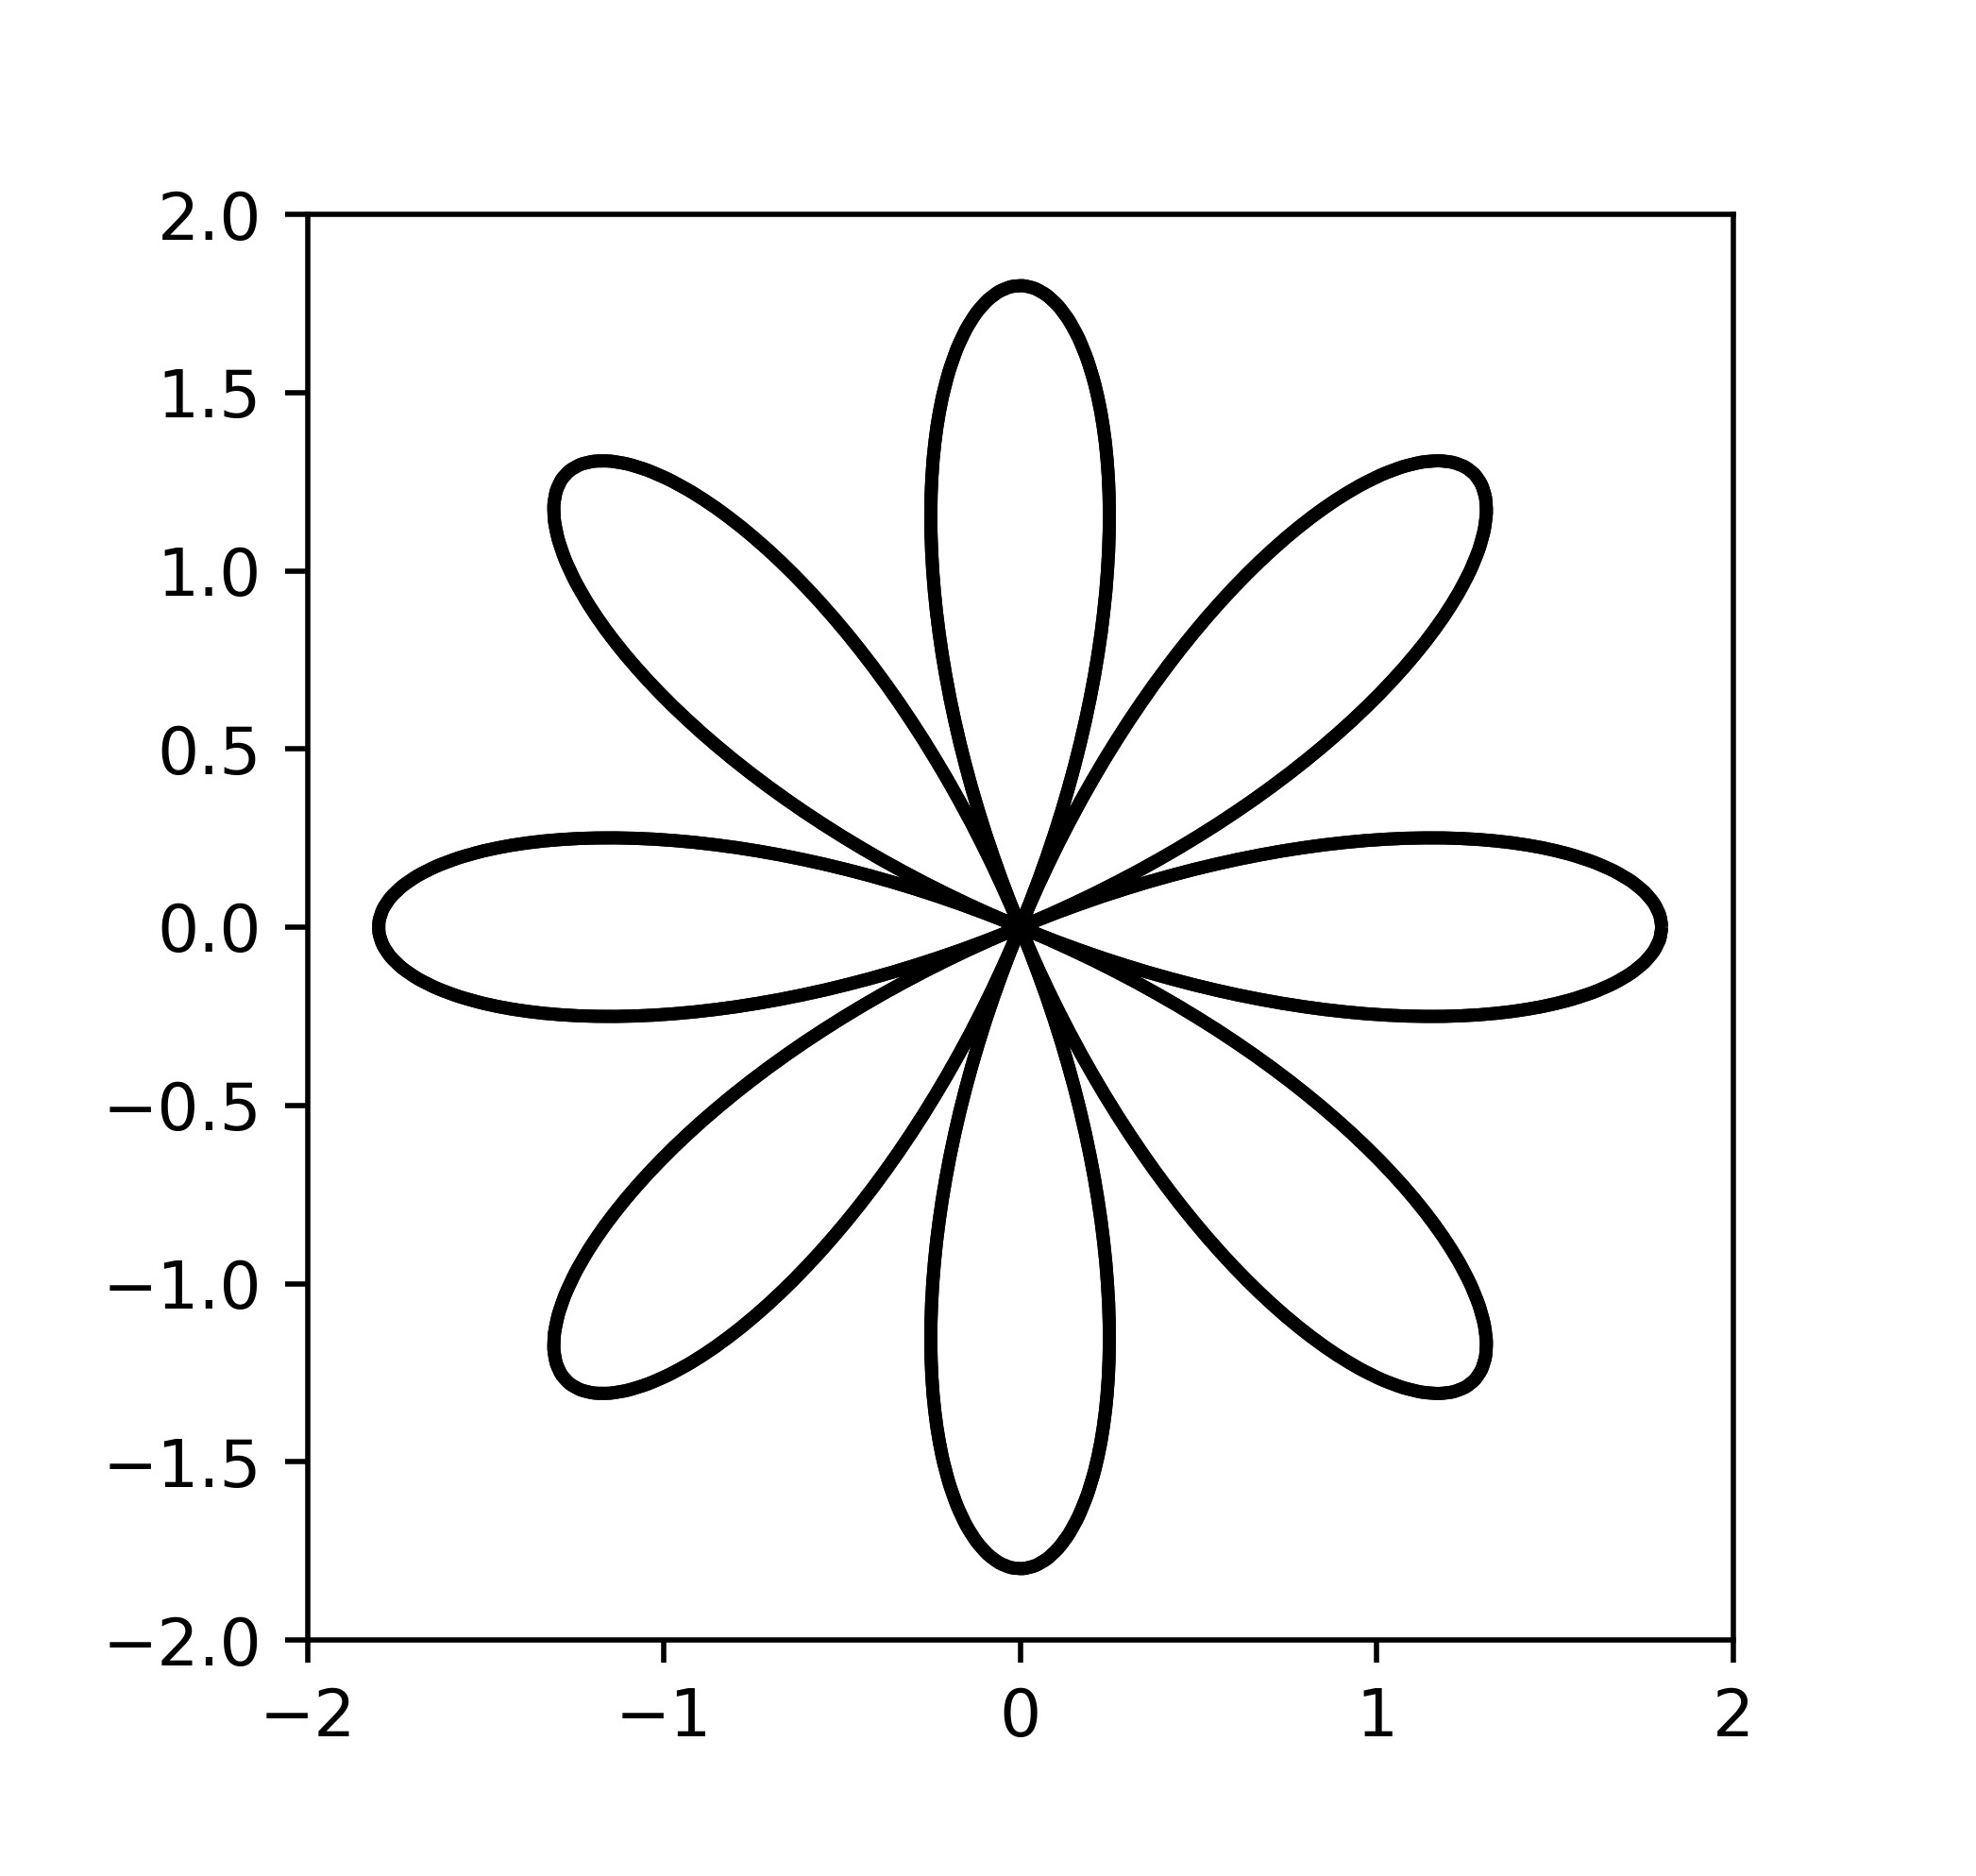
\includegraphics[width=7.5cm]{cartflower} }}%
    \qquad
    \subfloat[\centering Polar Plane]{{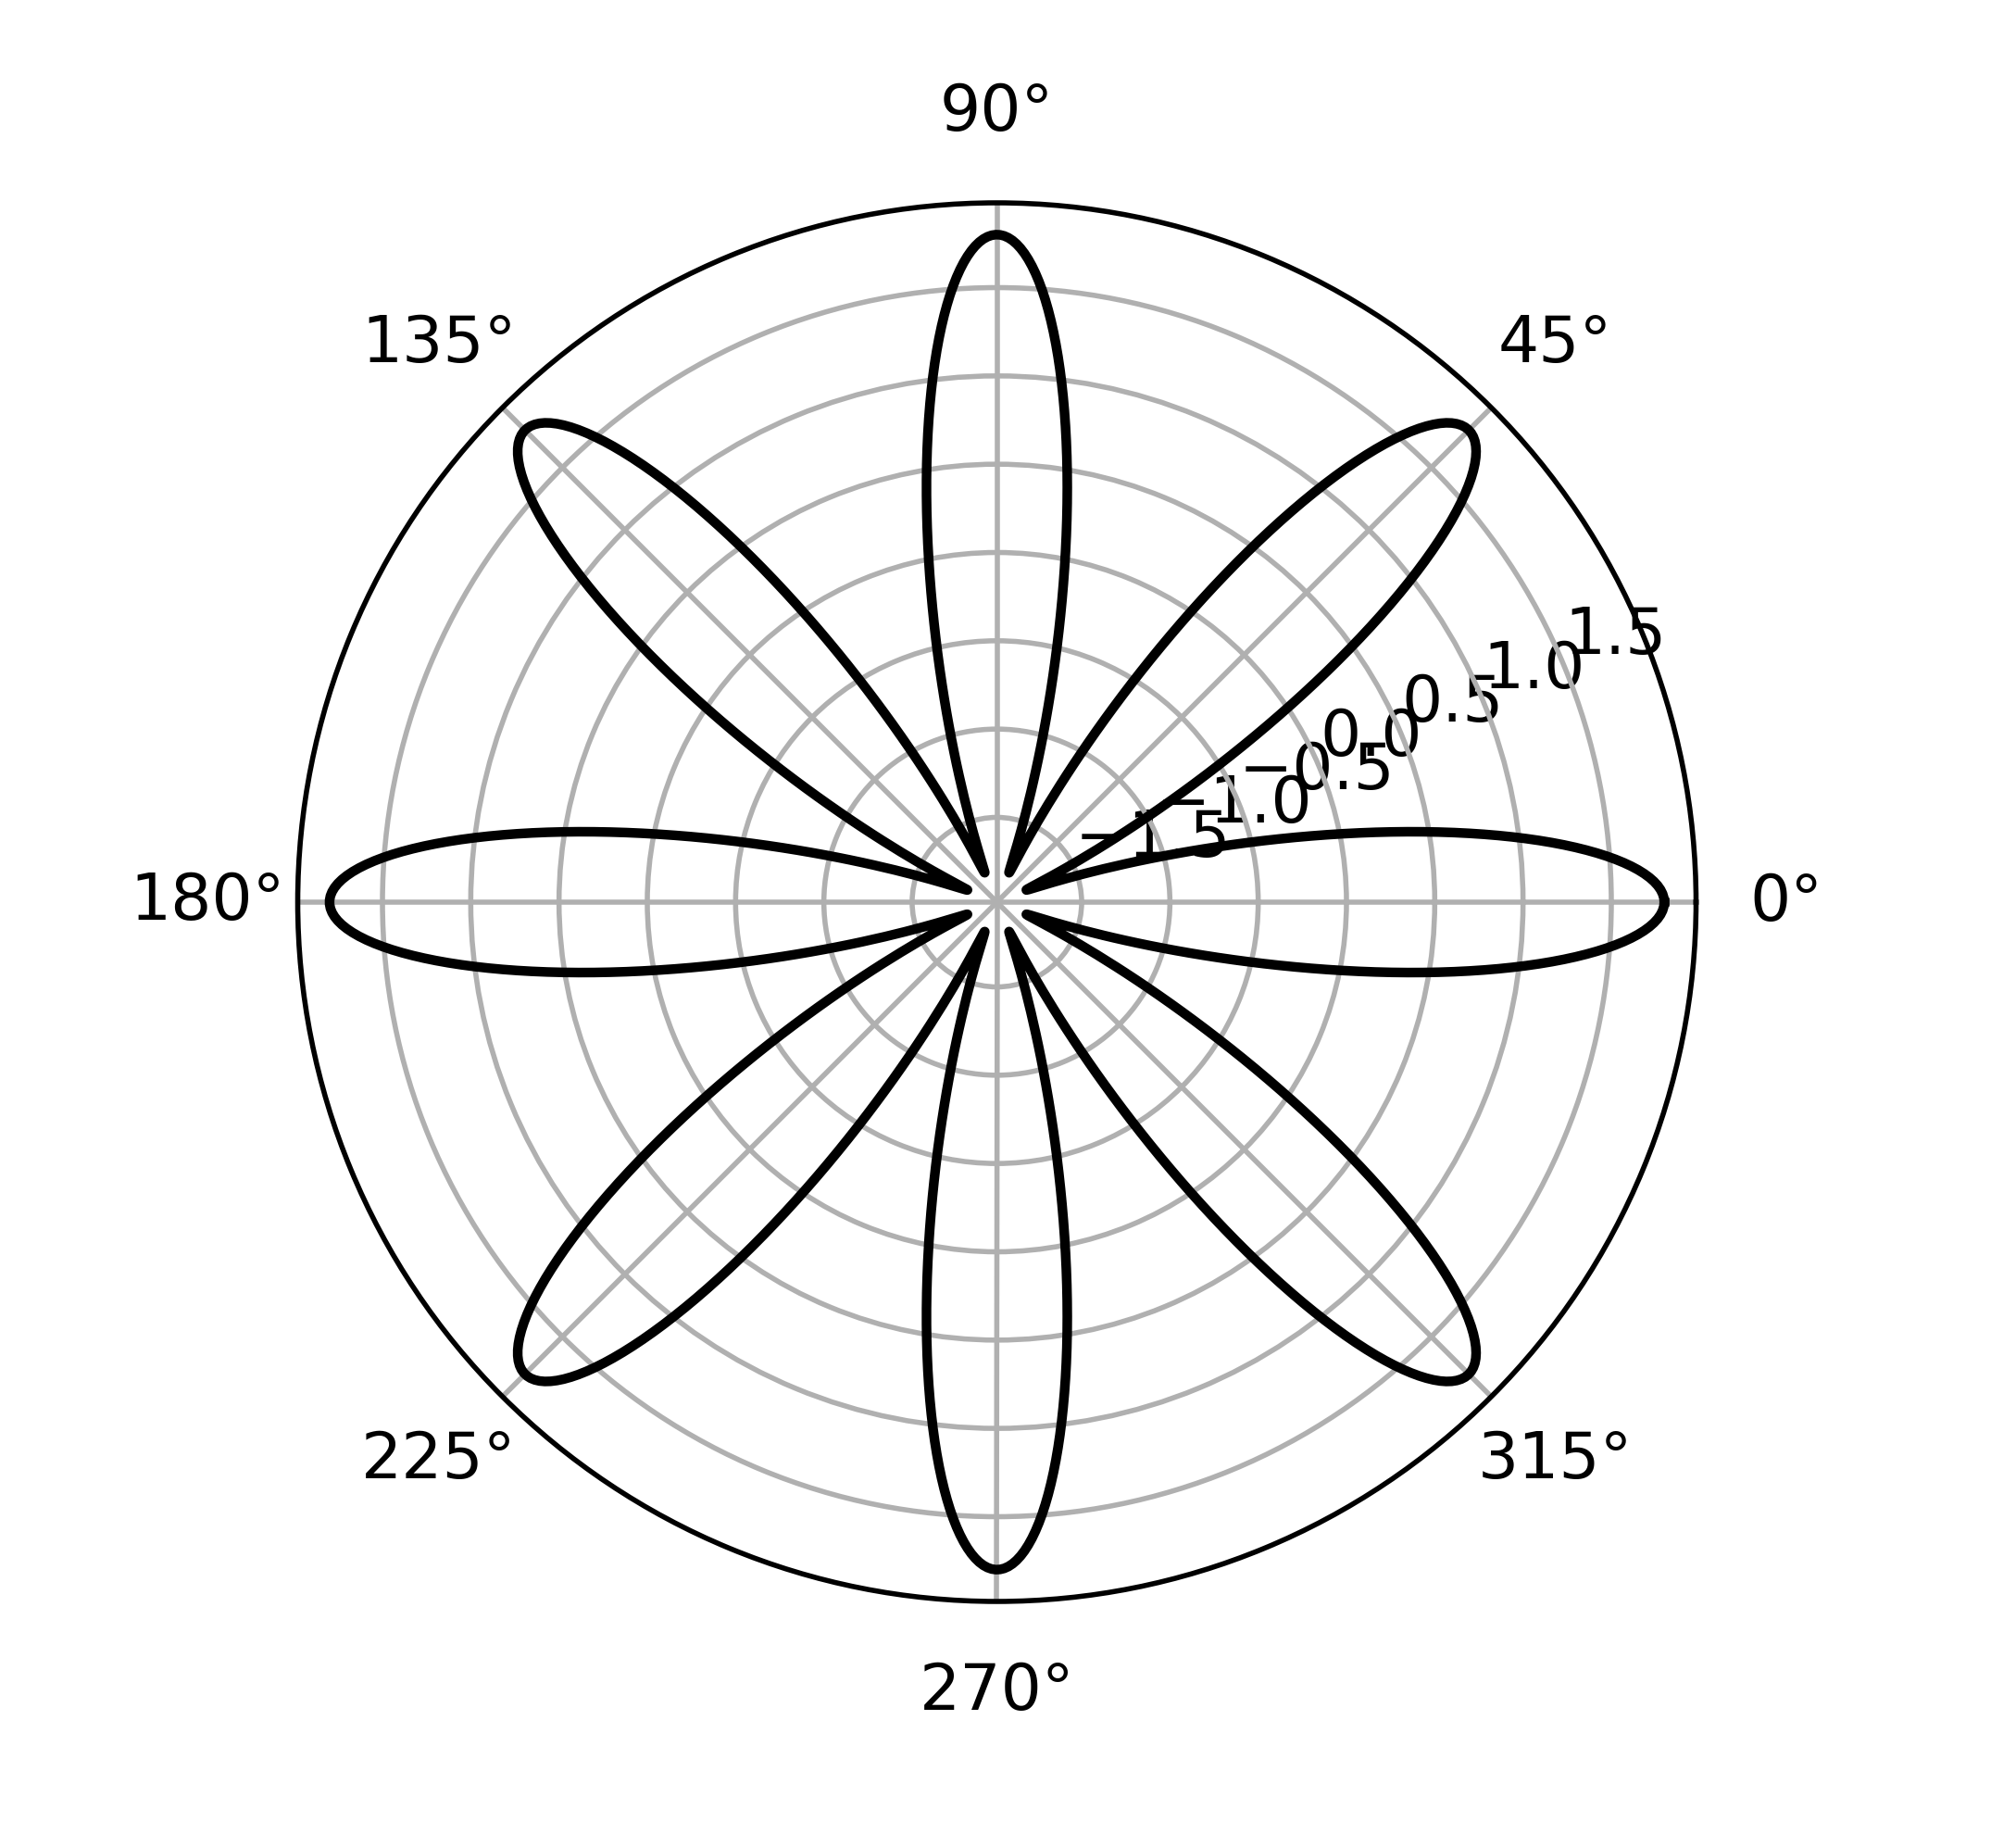
\includegraphics[width=7cm]{polarflower} }}\\[3ex]%
    \footnotesize{Figure 4: A Polar Rose graphed in two different planes (generated by the program).}%
    \label{fig:example}%
\end{figure}
\newpage
\subsection{Deterministic Calculations}
The equation for the polar rose used in this investigation (Figure 4) is as follows:\\[-3ex]
\[r=1.8*\cos(4\theta)\]
In the equation, 1.8 means that each petal is 1.8 units long, and 4 stands for the number of petals per half of the unit circle. Additionally, the polar coordinate \emph{r} is the length of the line segment from a point (x,y) to the origin, and the coordinate $\theta$ is the angle of between this line segment and the positive x-axis. First, it is important to note that the entire shape is composed of duplicates of one petal, all of which are centered at the origin. This means that, to find the area of the whole shape, we simply need to find the area of one petal and multiply it by the total number of petals present. To derive a formula for this, a circle with radius \emph{r} will be considered. As mentioned prior, the standard area of a circle equation is\\[-2ex]
\[A=\pi r^2\]

Within this full circle (whose angle measures 2$\pi$), a sector subtending to an angle of $\theta$ would have an area of \\[-2ex]
\[\pi r^2 * \frac{\theta}{2\pi} = \frac{1}{2}r^2\theta\]

This produces a sinusoidal function in the Cartesian plane. Integrating this function over $\theta_1 \leq \theta \leq \theta_2$ yields the expression for the area swept out of the curve:
\[\boxed{A_{Petal} \approx \frac{1}{2}\int\limits_{\theta_1}^{\theta_2} r^2 \ d\theta }\]
This is the desired formula for the area of one pedal. Given this, as well as the dimensions of the rose provided by the formula, we can solve for the area of the pedal. Figure 4b informs us that two different pedals in quadrant 1 are bisected by $\theta=0$ and $\theta=\frac{\pi}{4}$. If the areas of these two half-petals are combined, they will form the area of one pedal. Thus, the bounds for the integral can be set as such, and $r$ can be substituted in to produce the formula representing the area of the function: \\[-2ex]
\[\frac{1}{2}\int\limits_{0}^{\frac{\pi}{4}} (1.8\cos(4\theta))^2 \ d\theta \]
The function can then be simplified and solved using integration:
\[\frac{1}{2}(1.8\cos(4\theta))^2 \approx \frac{1}{2}(1.8^2\cos^2(4\theta))\]
\[=\frac{81\cos^2(4\theta)}{50}\]


Step 1: Apply linearity to produce

\[\frac{81}{50}\int\limits_{0}^{\frac{\pi}{4}} (cos(4\theta)) \ d\theta \]

Step 2: Solve $\int \cos^2(4\theta) \ d\theta$ using u-substitution:

\[Substitute\; u=4\theta \rightarrow \frac{du}{d\theta} = 4 \rightarrow d\theta = \frac{1}{4}du\]
\[=\boxed{\frac{1}{4}\int \cos^2(u)\ du}\]

Step 3: Apply reduction formula for $\int \cos^2(u) \ du$:
\[\int \cos^n(u) \ du=\frac{n-1}{n}\int \cos^{n-2}(u) \ du + \frac{\cos^{n-1}(u)\sin(u)}{n}\]
\[Set \ n=2\]
\[=\frac{\cos(u)sin(u)}{2} + \frac{1}{2} \int 1 \ du\]

Step 4: Solve $\int 1 \ du$

\[\int 1 \ du \rightarrow Apply \ constant \ rule:\]
\[= \boxed{u}\]

Step 5: Plug the two solved integrals into
\[\frac{\cos(u)\sin(u)}{2} + \frac{1}{2}\int 1 \ du\]
\[= \frac{\cos(u)\sin(u)}{2} + \frac{u}{2} \]
\[\therefore \ \frac{1}{4}\int \cos^2(u)\ du = \frac{\cos(u)\sin(u)}{8} + \frac{u}{8} \]

Step 6: Undo u-substitution by replacing \emph{u} with $4\theta$
\[=\frac{cos(4\theta)\sin(\theta)}{8} + \frac{\theta}{2}\]

Step 7: Plug back into initial integral, $\frac{81}{50}\int\limits_{0}^{\frac{\pi}{4}} (cos(4\theta)) \ d\theta $, from step 1
\[=\frac{80cos(4\theta)\sin(\theta)}{400} + \frac{81\theta}{100}\]

Step 8: Simplify and rewrite
\[\frac{81(\sin(8\theta)+8 \theta) + 80}{800} + C\]


When $\theta$ is replaced with $\frac{\pi}{4}$ in the solution to the integral (step 8), we get the area of one rose petal (Note: $C$ can be ignored because this integral is definite). This value can then be multiplied by 8 for the total area of the rose:

\[\frac{81 \pi}{400} * 8 = \boxed{5.0893 \ units^2}\]

\subsection{Solving Using the Monte Carlo Method}

The polar rose used in this investigation is in the Cartesian plane (Figure 4a) as opposed to the Polar plane (Figure 4b). This is done for the sake of consistency, as the circle from Section 2 is also in the Cartesian plane. Polar functions are plotted in the polar plane by default in Python; thus, the rose is first plotted in the polar plane using the aforementioned formula\\[-3ex]

\[r=1.8*\cos(4\theta)\]

This produces several thousand vertices that are subsequently connected via Bézier curves to form the closed shape (Figure 4b). Then, the program converts the coordinates of each polar point into its Cartesian equivalent through the following equations: \\[-3ex]

\[(r,\theta) \ \rightarrow \ (X_{Cartesian}, Y_{Cartesian})\]\\[-7ex]
\[\therefore\]\\[-7ex]

\[X_{Cartesian}=r*\cos(\theta)\]\\[-7ex]
\[Y_{Cartesian}=r*\sin(\theta)\]


\begin{figure}[h]
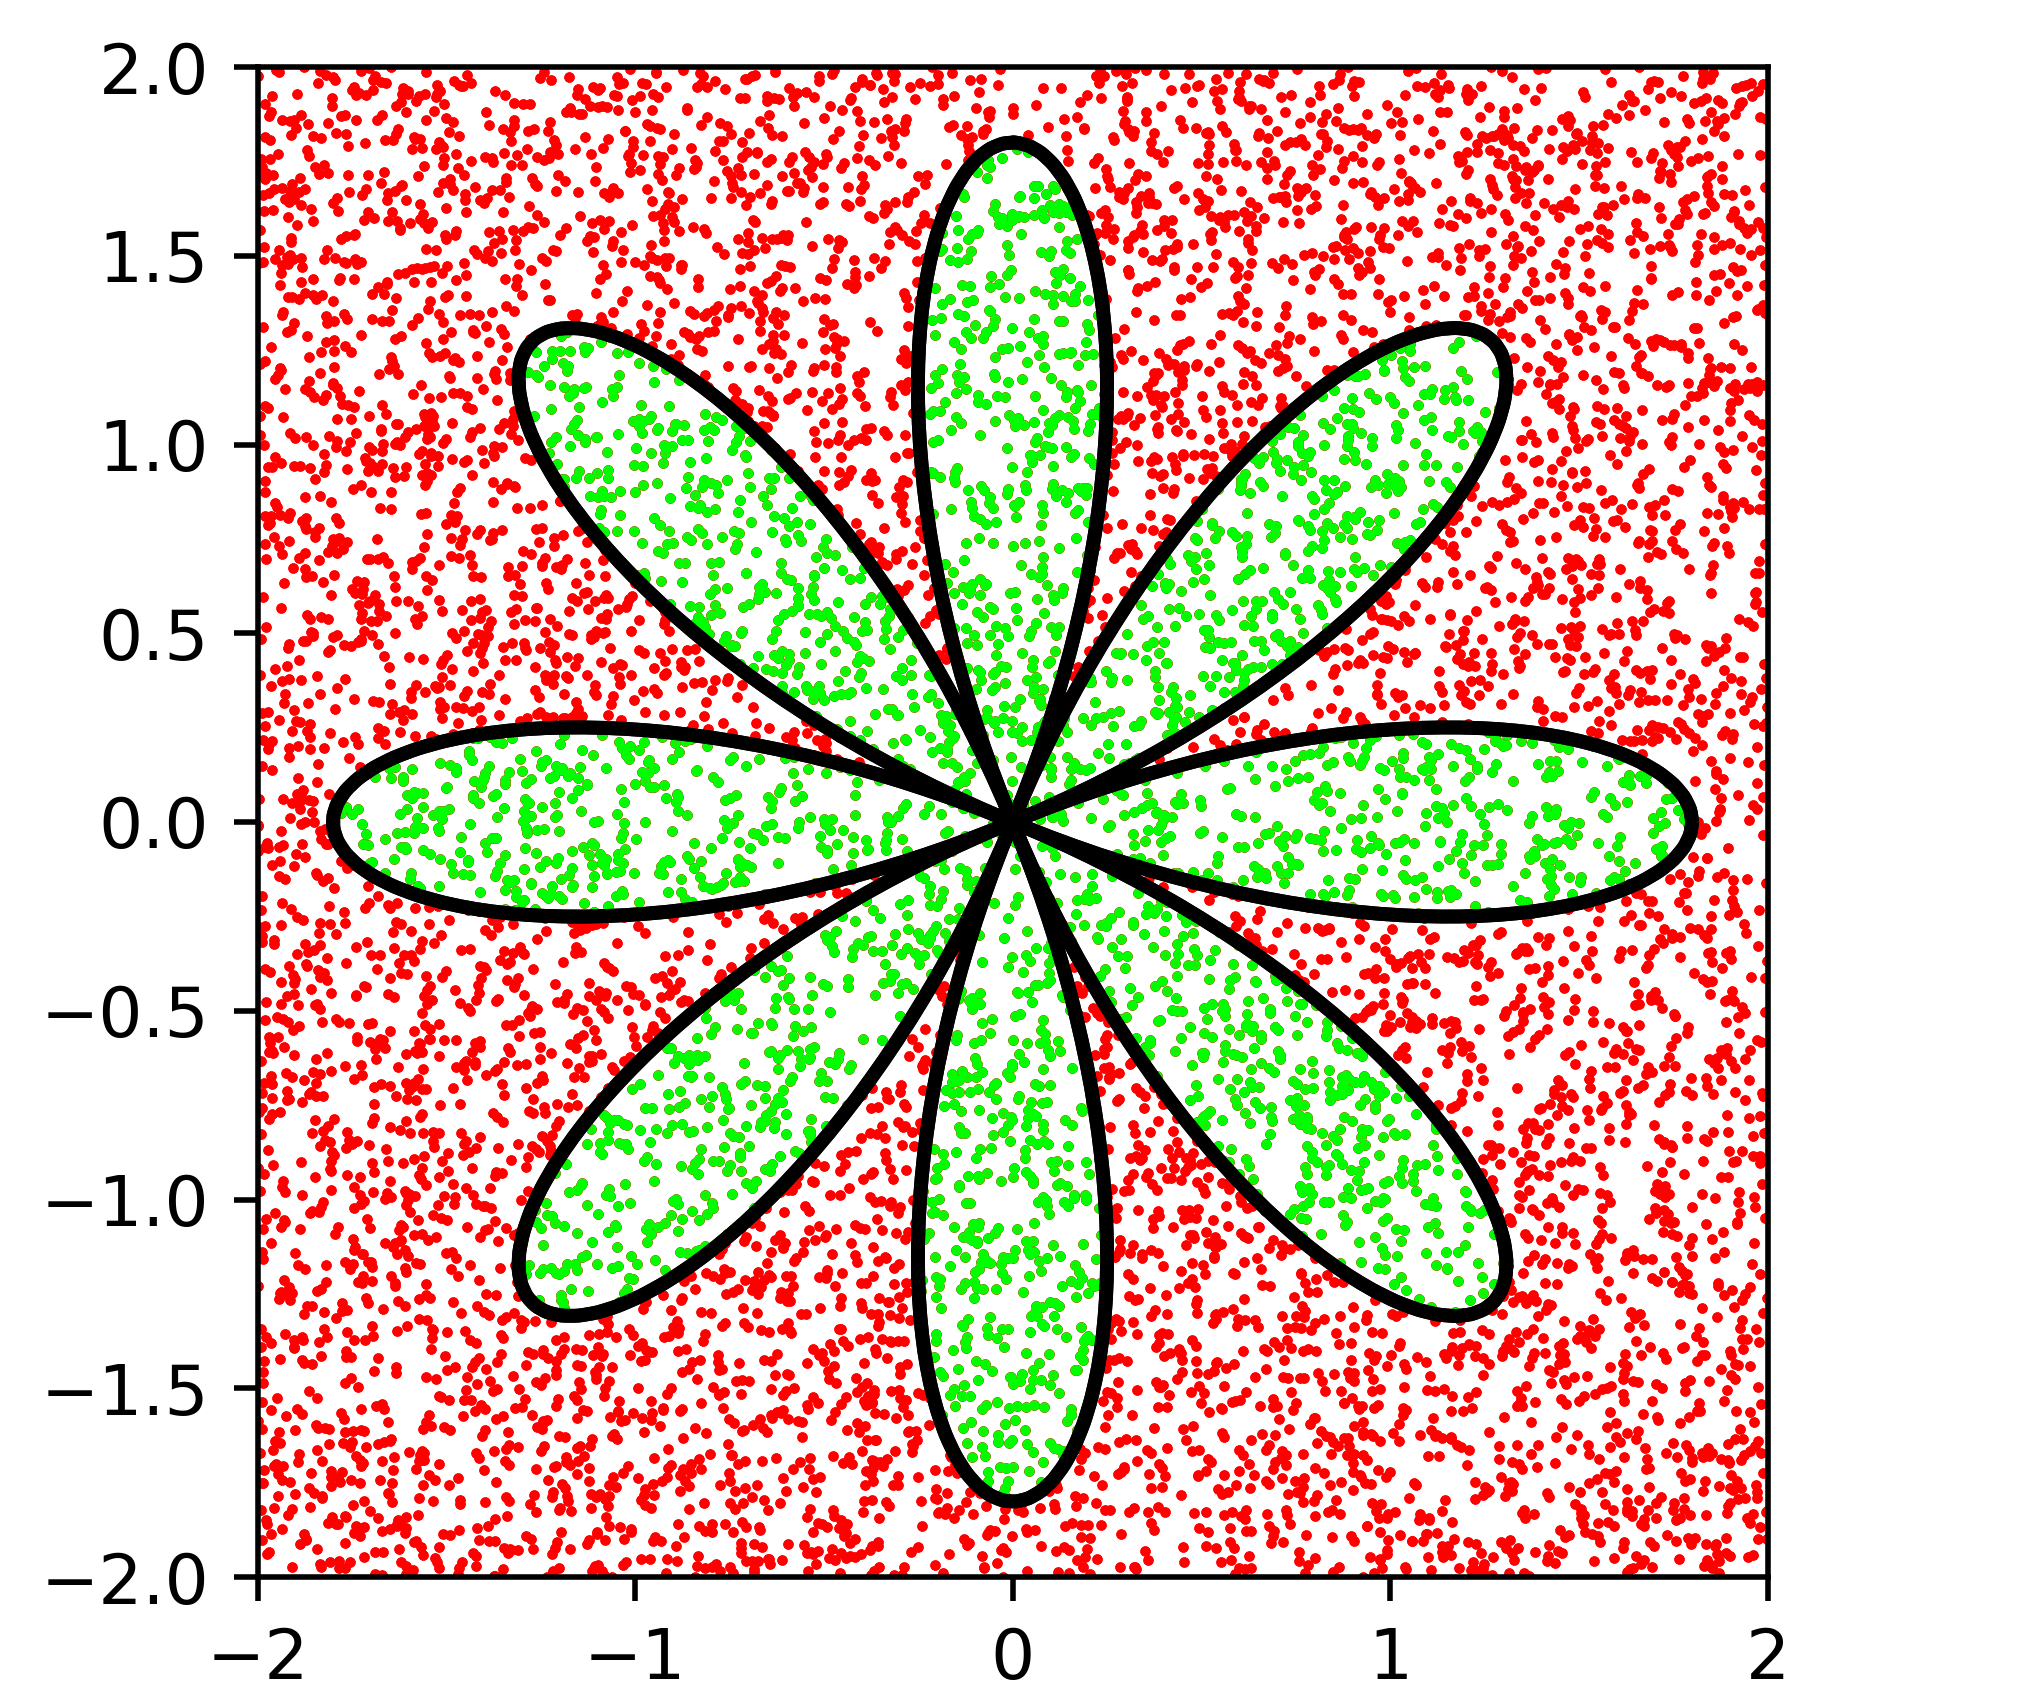
\includegraphics[scale=.2]{monte_carlo_rose}
\centering\\
\footnotesize\centering Figure 5: A visualization of the Monte Carlo simulation that solves for the area of the polar rose at 10,000 sample points.
\end{figure}

It took a computer 332 seconds to generate 100,000 points. As shown in Table 2, the percent error diminishes as more and more points are generated. At 100,000 data points, the percent error is negligible.

\begin{table}[H]
    \centering
    \begin{tabularx}{\linewidth}{>{\centering\arraybackslash}X>{\centering\arraybackslash}X>{\centering\arraybackslash}X>{\centering\arraybackslash}X>{\centering\arraybackslash}X }
      \hline \textbf{Number of Points} & \textbf{Points in Circle} & \textbf{Percent of Domain} & \textbf{Predicted Area} & \textbf{Percent Error} \\ \hline
              5                            &	3                         & 60.0\%                      & 9.6                  & 88.63\%            \\ \hline
              10                            &	5                        & 50.0\%                      & 8                  & 57.19\%            \\ \hline
              20                            &	8                        & 40.0\%                      & 6.4                  & 25.75\%            \\ \hline
              50                           &	13                        & 26.0\%                      & 4.16                  & 18.26\%            \\ \hline
              100                           &	30                       & 30.0\%                      & 4.8                  & 5.69\%            \\ \hline
              500                          &	163                       & 32.6\%                      & 5.216                  & 2.49\%            \\ \hline
              1000                          & 333                      & 32\%                      & 5.12                  & 0.6016\%            \\ \hline
              10000                          & 3168                      & 31.68\%                      & 5.0688                  & 0.4044\%            \\ \hline
              50000                         & 15932                      & 31.864\%                      & 5.09824                  & 0.1741\%            \\ \hline
              100000                         & 31807                     & 31.807\%                      & 5.08912                  & 0.00510\%            \\ \hline

    \end{tabularx}\\[2ex]
    \centering\footnotesize Table 2: Predicted area and its accuracy for a varying number of test points.
    \label{tab:data}
  \end{table}

Therefore, it can be said that, in this example, where the area of the polar rose is calculated, it is much simpler and less time-consuming to use the Monte Carlo method rather than using integration to solve the area of the shape. Setting up the expression, determining the limits of integration, and solving requires a hefty amount of calculation, whereas generating 100,000 points with a computer program that runs a Monte Carlo simulation produced the same answer of $5.0891 \ units^2$ in far less time (although there is a degree of error, it is negligible). Thus, for finding the area of complex shapes, using the Monte Carlo method is clearly the advantageous method of calculation.

\section{Applications}

Evidently, using the Monte Carlo method to solve for area is advantageous when performing complex mathematical calculations. Thus, the Monte Carlo method can provide a viable alternative to calculating the volume of complex 3D shapes in Euclidean geometry deterministically as well, as its computational process is dramatically more complicated than of calculating the area of complex 2D shapes. The Monte Carlo method has many applications in the real world as well. In engineering fields like automotive design, Monte Carlo simulation programs are used for geometric tolerancing, which verifies that parts will assemble in all variant part conditions. Tolerance is the total amount that dimensions in a part may vary from a specific value in order for all parts to still be able to assemble. Such programs then use the Monte Carlo method to generate a vast number of assemblies, each of which is composed of parts with dimensions that vary slightly from what is considered "perfect." This enables engineers to make a better-informed decision when selecting an assembly to manufacture (this tolerance range is important during the manufacturing process, as no machined part is perfect; thus, typically, the assembly with the larger tolerance range is selected). \cite{catia}\\[3ex]

Additionally, Monte Carlo simulations are used in economics to predict the future performance of markets given historical data. One such example of a market performance predictor that uses a Monte Carlo simulation is the application cFIRESim. This product considers Consumer Price Index inflation (the average change in price over time consumers pay for a good), the value of the user's portfolio, their retirement time frame, yearly spending, and yearly income to predict the geometric mean of the growth of the user's portfolio, and aid them in deciding whether to buy or sell stocks, and in managing their portfolio altogether. \cite{cfiresim} 

\section{Conclusion}
I began this investigation with the intention to investigate what allows 3D computer graphics software to accurately simulate light, as well as the Monte Carlo method (as I had never heard of it); however, I came out with much more. First, through taking a deep dive into the mathematics behind the Monte Carlo method, as well as the multitude of ways in which it has revolutionized the fields of science, economics, and engineering, I was able to learn more about the world. Second, this investigation provided me with an opportunity to link up my math coursework with my hobbies—graphic design and computer science—and learn new skills. Thus, due to what I learned, as well as the fact that the Monte Carlo method circumvents the deterministic relationship between computational time and problem complexity, I will use the Monte Carlo method in programs I write in the future to simplify calculations and improve performance.\\[3ex]

Altogether, I believe that through investigating Monte Carlo simulations, I have grown as a mathematician. Specifically, this investigation has taught me that, contrary to popular belief, creativity is involved in mathematics. In other words, I learned there is never one way to solve a mathematical problem, and that the conventional approach to solving a problem doesn't necessarily mean that it is the best approach. Thus, I have broadened my ability to solve deterministic problems in an unconventional manner (i.e. I have improved my critical thinking skills). That said, with my new knowledge, I can better appreciate the widespread application of mathematics in my daily life.


\newpage

\begin{thebibliography}{9}

\bibitem{blenderrender} 
Milan Jaroš, Lubomír Říha, Petr Strakoš, Tomáš Karásek, Alena Vašatová, et al.. Acceleration of Blender Cycles Path-Tracing Engine Using Intel Many Integrated Core Architecture. 14th Computer Information Systems and Industrial Management (CISIM), Sep 2015, Warsaw, Poland. pp.86-97, ff10.1007/978-3-319-24369-6\_7ff. ffhal-01444507f

\bibitem{pythongen} 
Random Generator. (n.d.). Retrieved April 01, 2021, from https://numpy.org/doc/stable/reference/random/generator.html


\bibitem{dynamicprogramming} 
Bellman, R. E. (2010). \emph{Dynamic Programming}. Princeton, NJ: Princeton University Press.

\bibitem{catia}
Catia V6 Integrated Tolerance and SPC Systems. (n.d.). Retrieved March 03, 2021, from https://www.3dcs.com/en-gb/tolerance-analysis-software-and-spc-systems/catia-v5-integrated\#:~:text=\\The\%20Leading\%20Variation\%20Analysis\%20Solution,\%2DMean\%20(Sensitivity)\%20Analysis.

\bibitem{cfiresim}
CFIRESim. (n.d.). Retrieved March 03, 2021, from https://www.cfiresim.com/


\end{thebibliography}

\newpage

\appendix


\section{Appendix: Python Code for the Monte Carlo Program}



\begin{singlespace}
\begin{lstlisting}
import numpy as np
import matplotlib.pyplot as plt
from matplotlib.patches import Circle
from matplotlib.path import Path
import matplotlib.patches as patches
import time

# Define timer

then = time.time()

# ==============================================
#                   SHAPES
# ==============================================

# ####################################
# #    Circle (uncomment to use)
# ####################################
# Create the initial circle
circle = Circle([-1,-1], radius=1)

# Get the path
path = circle.get_path()
patch = patches.PathPatch(path, facecolor='none', edgecolor='#000000')

## ####################################
## #   Polar Rose (uncomment to use)
## ####################################

# Plot in polar coordinates

theta = np.linspace(0, 2 * np.pi, 1000)  # generate 1000 points in a circle (hence 2pi)

r = 1.8 * np.cos(4 * theta)  # funtion

# convert to cartesian

xcart = r * np.cos(theta)
ycart = r * np.sin(theta)

newarrx = np.array_split(xcart, 1000)
newarry = np.array_split(ycart, 1000)

verts = [None] * 1000
codes = [None] * 1000

i = 0
while i < 1000:
    verts[i] = (float(newarrx[i]), float(newarry[i]))
    codes[i] = Path.CURVE4
    i = i + 1

codes[0] = Path.MOVETO

path = Path(verts, codes)

(fig, ax) = plt.subplots()
patch = patches.PathPatch(path, facecolor='none', lw=2)
ax.add_patch(patch)

##################
#  Scatter Plot
##################

# Total number of random points

total_random_points = 5

# Create empty x and y arrays for eventual scatter plot of generated random points

x_plot_array = np.empty(shape=(1, total_random_points))
y_plot_array = np.empty(shape=(1, total_random_points))

# Create random values (x,y) between -1 and 1

x = np.random.uniform(-2, 2, size=total_random_points)
y = np.random.uniform(-2, 2, size=total_random_points)

# Plot output of random points and circle

random_points_plot = plt.scatter(x, y, color='red', s=.25)
random_points_plot.set_zorder(0)  # set scatter plot position to back

# ==============================================
#           MONTE CARLO CALCULATIONS
# ==============================================

inside_shape = 0

# Iterate over points to locate them and count points inside unit circle

for i in range(0, total_random_points):

    # locates the points

    x_2 = x[i]
    y_2 = y[i]

    # Tests for whether the specified point is contained by the shape

    result = str(path.contains_points([[x_2, y_2]]))

    # Count if inside shape

    if '[ True]' == result:
        inside_shape = inside_shape + 1  # Add 1 to the counter
        plt.scatter(x[i], y[i], color='lime', s=.25)  # Change the color of the point to green

# Stats: Number of points inside shape compared to total

in_to_out_ratio = inside_shape / total_random_points

# ==============================================
#                    DRAW
# ==============================================
# Create axis with equal aspect ratio in both axis

ax = plt.gca()
ax.set_aspect('equal', 'box')

# Set axis limits

ax.set_xlim((-2, 2))
ax.set_ylim((-2, 2))

# Add the points and the shape to the plot

ax.add_artist(random_points_plot)
ax.add_patch(patch)

# Render plot in screen

plt.show()

# End timer

now = time.time()

# Log stats in console

print '\n--------------'
print '\n Statistics'
print ('\n Total number of points on graph:', total_random_points)
print ('\n Area of graph:', 16)
print ('\n IN OUT RATIO:', in_to_out_ratio)
print ('\n Number of points inside shape:', inside_shape)
print ('\n Area of shape:', in_to_out_ratio * 16)  # Multiplying probability by total area to find area of sector
print ('Calculation performed in: ', now - then, ' seconds')

\end{lstlisting}
\end{singlespace}



\end{document}
